\section{Theoretical Analysis}
\label{sec:theo}
\subsection{Mesh Analysis}
This circuit analysis method results from the application of Kirchhoff's Voltage Law (KVL) and it is based on loop currents flowing around meshes. The analysis is performed with a certain sequence of steps. First, we start by identifying the meshes and assigning a current to each of those, as it can be seen in Fig. \ref{fig:mesh_scheme}.

\begin{figure}[h]
    \centering
    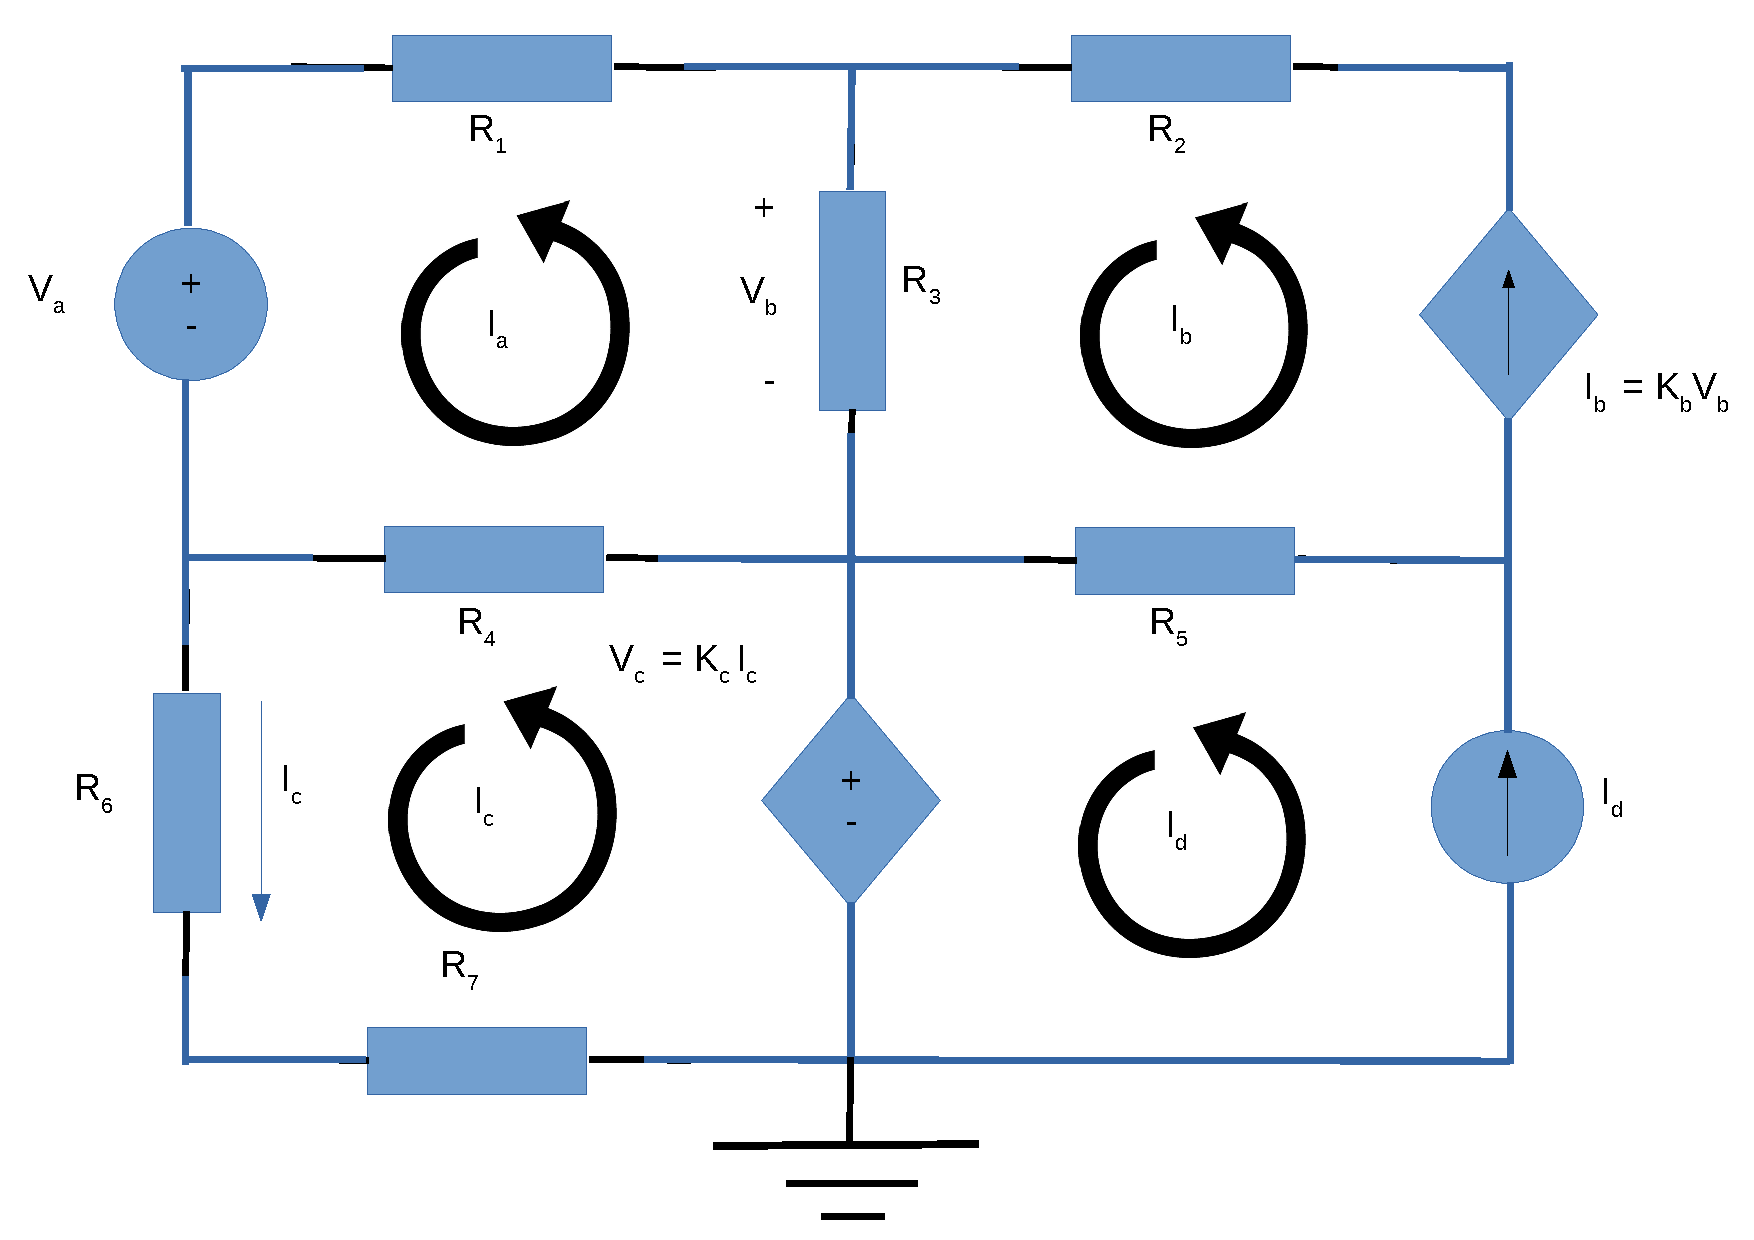
\includegraphics[width = 0.7\linewidth]{mesh.pdf}
        \caption{\textit{Mesh analysis scheme for this circuit that shows the adopted current direction for each mesh}}
    \label{fig:mesh_scheme}
\end{figure}

After that, the next step is to write linearly independent Kirchhoff's Voltage Law equations for each mesh that allows finding the unknown current values. For this circuit, as $I_d$ is known, and following the current directions represented in Fig. \ref{fig:mesh_scheme}, we obtained the following system of equations:

\begin{equation}
    \begin{cases}
        (R_1+R_4)I_a - (\frac{1}{K_b})I_b - R_4I_c = -V_a \hspace{15px} \text{(mesh A)}\\
        -R_4I_a + (R_4 + R_6 + R_7 - K_c)I_c = 0 \hspace{23px} \text{(mesh B)}\\
        R_3I_a + (\frac{1}{K_b}-R_3)I_b = 0 \hspace{45px} \text{(restriction involving meshes A and B)}
    \end{cases}
\end{equation}

Note that the restriction equation used as the third equation of the system of equation urges as a result of the resistor $R_3$ terminals voltage. One can write the voltage of the resistor $R_3$ as being defined by

\begin{equation}
    V_b = R_3 (I_b - I_a)
\label{Vb1}
\end{equation}

Furthermore, it is known from the equation associated with the dependent current source in mesh B, that the voltage $V_b$ can be defined as

\begin{equation}
    V_b = \dfrac{I_b}{K_b}
\label{Vb2}
\end{equation}

In fact, combining equations \eqref{Vb1} and \eqref{Vb2} one can obtain:

\begin{equation}
    R_3(I_b - I_a) = \dfrac{I_b}{K_b} \Longleftrightarrow R_3 I_a + \left(\dfrac{1}{K_b} - R_3\right) I_b = 0
\end{equation}

Converting this system of equations in its matricial form and using \textit{Octave} to solve it, we get that:

\begin{equation}
    \begin{bmatrix}
        R_1 + R_4 & -\frac{1}{K_b} & -R_4 \\
        -R_4 & 0 & R_4 + R_6 + R_7 - K_c \\
        R_3 & \frac{1}{K_b} - R_3 & 0
    \end{bmatrix} 
    \begin{bmatrix}
        I_a \\
        I_b \\
        I_c
    \end{bmatrix} =
    \begin{bmatrix}
        -V_a \\
        0 \\
        0
    \end{bmatrix} \Longleftrightarrow
    \begin{bmatrix}
        I_a \\
        I_b \\
        I_c
    \end{bmatrix} = 
    \input{"../mat/mesh_an"} mA
\label{eqmalhas}
\end{equation}

From this result, it is possible to infer that, according to the current directions assigned and represented in Fig.\ref{fig:mesh_scheme}, $I_a$ and $I_b$ flow in the clockwise direction while $I_c$ and $I_d$ (with positive signs) flow in the counterclockwise direction. To finish the mesh analysis of this circuit, we just need to use the current values obtained in \eqref{eqmalhas} to calculate what is still left unknown in the circuit:

\begin{equation}
    V_c = K_c I_c \Longleftrightarrow V_c = \input{"../mat/vc"}V
\end{equation}

\begin{equation}
    V_b = (I_b - I_a) R_3 = -0.040292V
\end{equation}

\subsection{Nodal Analysis}

Let $\Vec{b} = [V_1, V_2, V_3, V_4, V_5, V_6, V_7, I_a, I_c]$, such that $[V_i] = V$, $[I_i] = A$. For the nodes, we used the ones given in Fig. \ref{fig:nodal_scheme}, as well as the currents there presented. 

\begin{figure}[h]
    \centering
    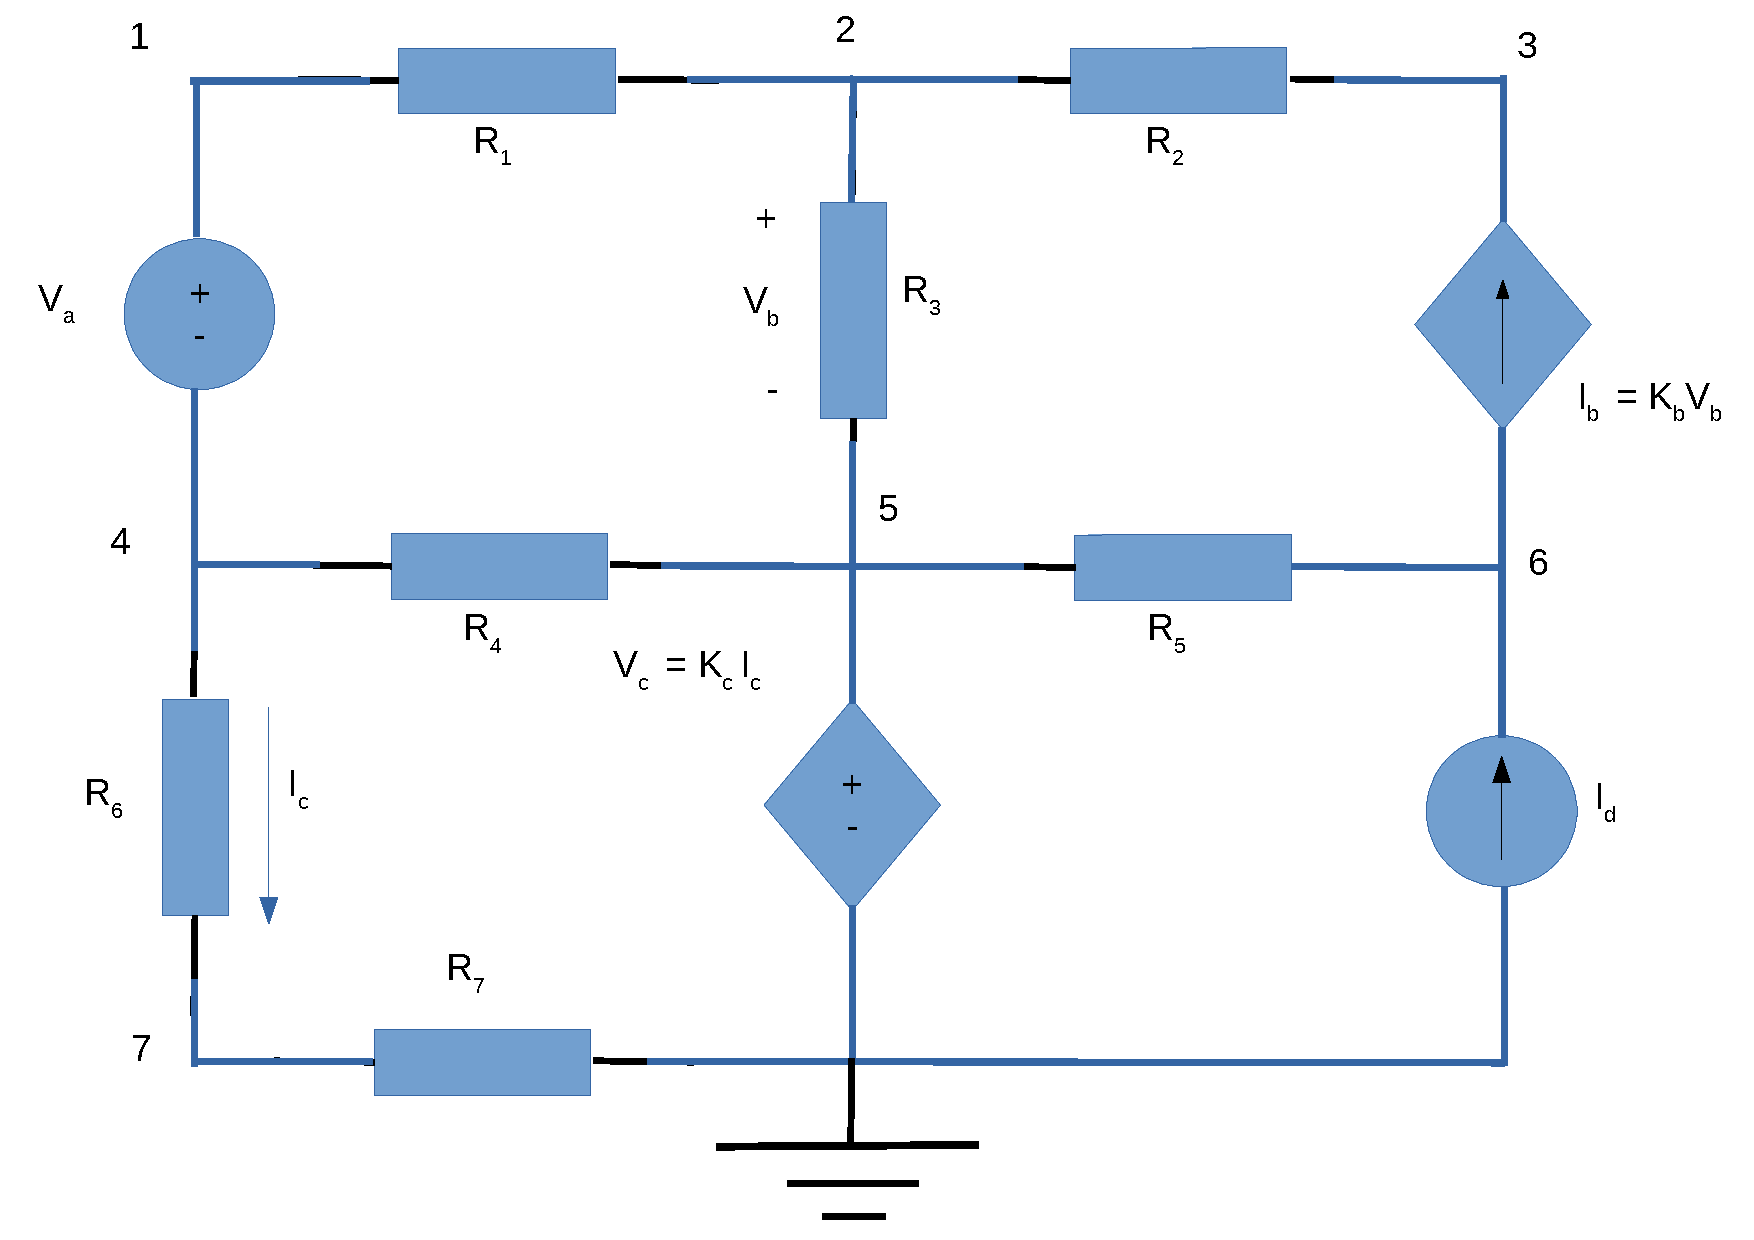
\includegraphics[width = 0.7\linewidth]{nodal.pdf}
        \caption{\textit{Nodal analysis scheme for this circuit that shows the labels given to each of the circuit's nodes}}
    \label{fig:nodal_scheme}
\end{figure}

Thus, for each node, we get the following linearly independent equations (as it was supposed, we obtained 7 linearly independent equations for a circuit with 8 nodes),

\begin{equation}
    \begin{cases}
        G_1(V_1 - V_2) + I_a = 0 \hspace{15px} \text{(node 1)}\\
        G_1(V_2 - V_1) + G_2(V_2 - V_3) + G_3(V_2-V_5) = 0 \hspace{15px} \text{(node 2)}\\
        G_2(V_3 - V_2) - K_b(V_2 - V_5) = 0 \hspace{15px} \text{(node 3)}\\
        G_4(V_4 - V_5) + G_6(V_4 - V_7) - I_a = 0 \hspace{15px} \text{(node 4)}\\
        G_3(V_5 - V_2) + G_4(V_5 - V_4) + G_4(V_5 - V_6) - I_c = -I_d \hspace{15px} \text{(node 5)}\\
        G_5(V_6 - V_5) + K_b(V_2 - V_5) = I_d \hspace{15px} \text{(node 6)}\\
        G_6(V_7 - V_6) + G_7(V_7 - V_8) = 0 \hspace{15px} \text{(node 7)}\\
    \end{cases}
\end{equation}

Note that node 8 will have null voltage, $V_8=0$, because ground (GND) was assigned to it. Furthermore, by inspection (and it is pretty clear from the scheme presented in Fig.\ref{fig:nodal_scheme}), one can also conclude that:

\begin{equation}
    \begin{cases}
        V_1 - V_4 = V_a\\
        V_5 - K_cI_c = 0\\
    \end{cases}
\end{equation}

Thus, having as many equations as variables, one can now solve this system (\ref{eqnodos}), using \textit{Octave}.

\begin{equation}
    \begin{bmatrix}
     G1 &  -G1      &  0 &    0  &     0      &  0  &  0    &  1 &   0\\
     -G1 & G1+G2+G3 & -G2  & 0   &  -G3       &  0  &  0    &  0 &   0\\
     0   & -G2-Kb    & G2  & 0   &   Kb       &  0  &  0    &  0 &   0\\
     0   & 0        & 0   & G4+G6 & -G4       &  0  & -G6   & -1 &   0\\
     0   & -G3      &  0 &  -G4  &   G3+G4+G5 & -G5 &  0    & 0  &  -1\\
     0   & Kb       & 0  &  0    & -G5-Kb     & G5  & 0     & 0  &   0\\
     0   & 0        & 0  & -G6   &  0         & 0   & G6+G7 & 0  &   0\\
     1   & 0        & 0  & -1    &  0         & 0   & 0     & 0  &   0\\
     0   & 0        & 0  &  0    &  1         & 0   & 0     & 0  & -Kc
    \end{bmatrix} 
    \Vec{b}
    = 
    \begin{bmatrix}
        0\\
        0\\
        0\\
        0\\
        -I_d\\
        I_d\\
        0\\
        V_a\\
        0
    \end{bmatrix}
\label{eqnodos}
\end{equation}

The matrix system \ref{eqnodos} is composed of a very sparse matrix, thus we also advise using correspondingly adapted sparse matrix solvers if possible, but this is already out of the scope of this discipline and laboratory. Getting back to the point, the solution to the matrix system is,

\input{"../mat/nodal_an"}

which produces, $V_c = \input{"../mat/vc_nodal"}V$, $V_b = \input{"../mat/vb_nodal"}V$, as expected.